\documentclass{standalone}

\usepackage{circuitikz}
\usepackage{newtxtext}
\usepackage{newtxmath}

\begin{document}
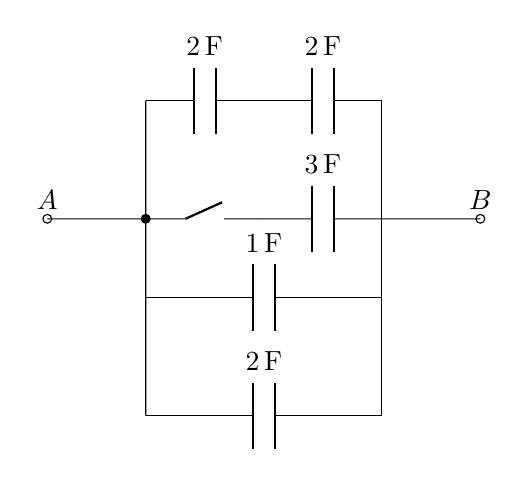
\begin{tikzpicture}[transform shape]
	\draw (3, 6) to[capacitor, l={$2\,\mathrm{F}$}] (4.5, 6);
	\draw (4.5, 6) to[capacitor, l={$2\,\mathrm{F}$}] (6, 6);
	\draw (4.5, 4.5) to[capacitor, l={$3\,\mathrm{F}$}] (6, 4.5);
	\draw (6, 3.5) to[capacitor, l_={$1\,\mathrm{F}$}] (3, 3.5);
	\draw (3, 2) to[capacitor, l={$2\,\mathrm{F}$}] (6, 2);
	\draw (3, 4.5) to[normal open switch, *-] (4.5, 4.5);
	\node[ocirc](N1) at (1.75, 4.5){} node[anchor=south] at (N1.text){$A$};
	\node[ocirc](N2) at (7.25, 4.5){} node[anchor=south] at (N2.text){$B$};
	\draw (1.75, 4.5) to[short] (3, 4.5);
	\draw (6, 4.5) to[short] (7.25, 4.5);
	\draw (3, 6) to[short] (3, 2);
	\draw (6, 6) to[short] (6, 2);
\end{tikzpicture}
\end{document}